

\section{Density Functional Theory}

Density Functional Theory (DFT) is a branch of quantum chemistry that approximately solves the Schrӧdinger equation using electron density, rather than the coordinates of each electron in the system.  A number of simplifications are also applied in order for DFT to be practical to use, but despite this calculations are limited to just hundreds or thousands of atoms.  A calculation of a hundred or so atoms may take thousands of CPU hours at the time of writing, depending on the type of calculation and complexity of the electron structures of the atoms involved.

It is through DFT that the first principles energy, stress and force calculations will be made, and it's these results that the EAM potentials will be trained and fit to using the force matching method.  This will allow much larger scale modelling using the extrapolated behaviour of accurate DFT calculations.



\subsection{Brief Overview of DFT}


\begin{figure}[!h]
\centering
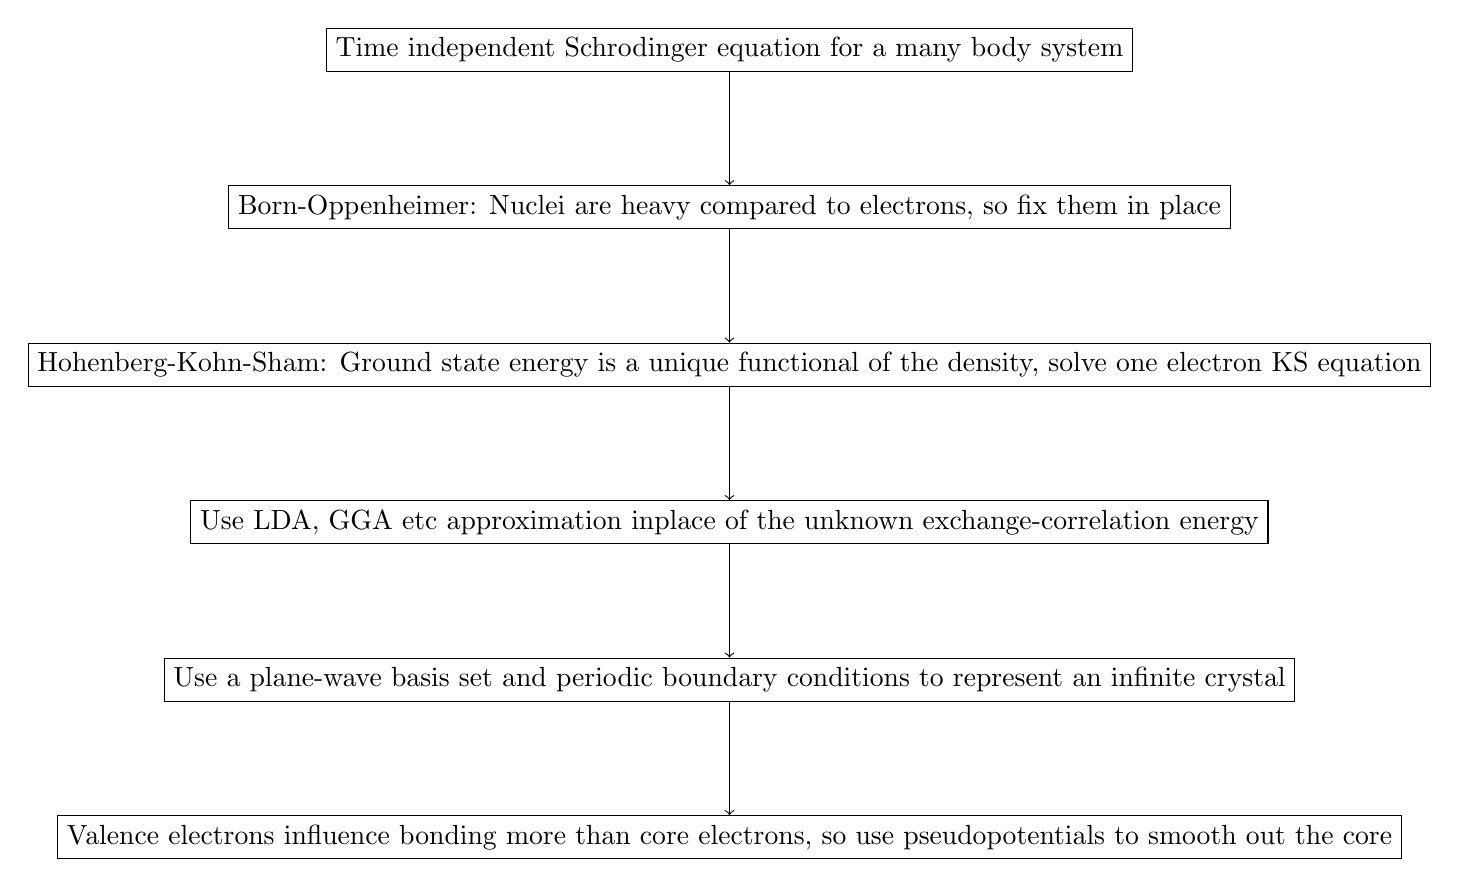
\begin{tikzpicture}[node distance=2cm]
\node (a) [rectangle, draw, fill=none] {Time independent Schrodinger equation for a many body system};
\node (b) [rectangle, draw, fill=none, below of=a] {Born-Oppenheimer: Nuclei are heavy compared to electrons, so fix them in place};
\node (c) [rectangle, draw, fill=none, below of=b] {Hohenberg-Kohn-Sham: Ground state energy is a unique functional of the density, solve one electron KS equation};
\node (d) [rectangle, draw, fill=none, below of=c] {Use LDA, GGA etc approximation inplace of the unknown exchange-correlation energy};
\node (e) [rectangle, draw, fill=none, below of=d] {Use a plane-wave basis set and periodic boundary conditions to represent an infinite crystal};
\node (f) [rectangle, draw, fill=none, below of=e] {Valence electrons influence bonding more than core electrons, so use pseudopotentials to smooth out the core};
%% arrows
\draw [->] (a) -- (b);
\draw [->] (b) -- (c);
\draw [->] (c) -- (d);
\draw [->] (d) -- (e);
\draw [->] (e) -- (f);
\end{tikzpicture}
\caption{Caption}
\label{fig:decaychain}
\end{figure}



Several important theories and approximations are used by DFT with the aim of calculating and minimising energies and forces.  The Born-Oppenheimer approximation separates the electron-nucleus wave function.  It treats the nuclei as fixed points, and the system of electrons in a fixed potential created by the nuclei.

 the DFT of Kohn, Sham and Hohenburg proved that the potential of a system is uniquely determined by its ground state density.  This makes solving the Schrodinger equation significantly easier.




\subsection{Time Independent Schrodinger Equation}

The Schrodinger equation is a linear partial differential wave equation, and it was proposed by Erwin Schrodinger in 1925.  There is a time-dependent and time indepent form of the equation, and as the DFT calculations in this work are static, only the time-independent version will be discussed.  

\begin{equation}
\begin{split}
\hat{H} \lvert \Psi \rangle = E \lvert \Psi \rangle
\end{split}
\label{eq:eqTimeIndependentSchrodinger}
\end{equation}

The Hamiltonian $\hat{H}$ is an operator, and it is the total energy in the system.  $Psi$ is the wave function (for example, the wavefunction of an electron) and this contains all the measureable information possible about whatever it represents.  E is the energy eigen value of this system and this will depend on the eigenstate of the system.  The wavefunction is also connected to the probability of a particle being found at a certain point in space, and the integral over all space is equal to 1 i.e. the probability of it being found somewhere in space is equal to 1.

\begin{equation}
\begin{split}
\int_{-\infty}^{\infty} \int_{-\infty}^{\infty}  \int_{-\infty}^{\infty}  \Psi(x,y,z) dx dy dz
\end{split}
\end{equation}

The Schodinger equation is set up depending on the system being studied.  Starting with the simplest, a free particle, the only non zero energy of then Hamiltonian is kinetic.


\begin{equation}
\begin{split}
\hat{H} = \frac{\hbar^2}{2 m} \nabla^2 \\
-\frac{\hbar^2}{2 m} \nabla^2 \Psi(\vec{r}) = E \Psi(\vec{r})
\end{split}
\label{eq:eqTimeIndependentSchrodinger}
\end{equation}

If the particle is in a potential, it will have both kinetic energy $\hat{T}$ and potential energy $\hat{V}$.

\begin{equation}
\begin{split}
\hat{H} = \hat{T} + \hat{V} = \frac{\hbar^2}{2 m} \nabla^2 + V(\vec{r})\\
\left[-\frac{\hbar^2}{2 m} \nabla^2 \right] \Psi(\vec{r}) = E \Psi(\vec{r})
\end{split}
\label{eq:eqTimeIndependentSchrodinger}
\end{equation}




\subsection{Many Body TISE}

Electronic structure calculations are important and allow the calculation of material properties that may be difficult or impossible to measure with current technology.  The next step is to set up the Schrodinger equation (time-independent) for nuclei and electrons in a crystal.  Relative to the strong force, the electromagnetic force is 1/137th as strong, but the strong force acts over a range of approximately $1.0 \times 10^{-5}$ angstrom.  In the calculations carried out in this section, the atoms will never be arranged close enough for the strong force to be considered at all.  The gravitational force, as with the electromagnetic force, acts over an infinite range.  The electromagnetic force is more than $1.0 \times 10^36$ times greater than the gravitational force, so it too can be neglected.  Finally, the weak interacting force has a range of approximately $1.0 \times 10^{-8}$ angstrom which, as with the strong force, is a range small enough that the weak force may be neglected.

The energy operators required are kinetic and electromagnetic potential.

\begin{equation}
\begin{split}
\hat{H} = \hat{T_e} + \hat{T_n} + \hat{V_{e-e}} + \hat{V_{e-n}} + \hat{V_{n-n}}
\end{split}
\label{eq:eqTimeIndependentSchrodinger}
\end{equation}

The first two terms are the kinetic energy of the electrons and nuclei respectively.

\begin{equation}
\begin{split}
\hat{T_e} = - \sum_{i} \frac{\hbar^2}{2 m}  \nabla^2 \text{Sum of kinetic energy of electrons} \\
\hat{T_n} = - \sum_{k} \frac{\hbar^2}{2 M}  \nabla^2 \text{Sum of kinetic energy of nuclei}
\end{split}
\label{eq:eqTimeIndependentSchrodinger}
\end{equation}

The last three terms are potential energy terms due to the electromagnetic force: 

\begin{equation}
\begin{split}
V_{e-e} = \frac{1}{2} \sum_{i,j,i \neq j} \frac{1}{\abs{\vec{r}_i - \vec{r}_j}} \text{sum of potential energy between electrons} \\
V_{e-n} = \sum_{i,k} \frac{z_i}{\abs{\vec{r}_i - \vec{r}_l}} \text{sum of potential energy between electrons and nuclei} \\
V_{n-n} = \frac{1}{2} \sum_{k,l,k \neq l} \frac{z_k z_l}{\abs{\vec{r}_l - \vec{r}_k}} \text{sum of potential energy between nuclei}
\end{split}
\label{eq:eqTimeIndependentSchrodinger}
\end{equation}

These operators are now input into the TISE.


\begin{equation}
\begin{split}
\left[ \left(- \sum_{i} \frac{\hbar^2}{2 m} - \sum_{k} \frac{\hbar^2}{2 M} \right) \nabla^2  + \sum_{i,k} \frac{z_i}{\abs{\vec{r}_i - \vec{r}_l}} + \frac{1}{2} \left( \sum_{i,j,i \neq j} \frac{1}{\abs{\vec{r}_i - \vec{r}_j}} + \sum_{k,l,k \neq l} \frac{z_k z_l}{\abs{\vec{r}_l - \vec{r}_k}} \right) \right] \lvert \Psi \rangle = E \lvert \Psi \rangle
\end{split}
\label{eq:eqTimeIndependentSchrodinger}
\end{equation}



\subsection{Born-Oppenheimer}

The TISE arrived at is far too complicated to solve, even for the simplest of systems.  It represents the many body system of electrons and nuclei, and the variables it takes are the positions of all nuclei and electrons.

\begin{equation}
\begin{split}
\hat{H} \lvert \Psi (\vec{r_e}, \vec{r_n}) \rangle = E \lvert \Psi (\vec{r_e}, \vec{r_n}) \rangle \\
\text{ where } \vec{r_e} = r_{e,1}, r_{e,1},...,r_{e,i} \text{ (electron positions)} \\
\text{ where } \vec{r_n} = r_{n,1}, r_{n,1},...,r_{n,i} \text{ (electron positions)} \\
\end{split}
\label{eq:eqTimeIndependentSchrodinger}
\end{equation}

In 1927 the Born-Oppenheimer approximation was proposed to seperate the electron components from the nuclei in the Hamiltonian.  

Protons and Neutrons are almost 2,000 times the mass of electrons.  With respect to the electrons, they move much slower and may be considered to be fixed or frozen in place.  Simplifying for a moment to a single electron and proton, due to Newton's second law, we can see that the acceleration of the electron would be similarly 2,000 times that of the proton: $f_e = f_p$ and $m_e a_e = m_p a_p$ which leads to $a_e = \frac{m_p}{m_e} a_p$.  As the nuclei move, the electrons are assumed to respond instantly, remaining in the ground state and not being promoted into higher energy levels.

The Hamiltonian of the electrons may be written with the electron co-ordinates as a variable, and the nuclei co-ordinates as a parameter.

\begin{equation}
\begin{split}
\hat{H_e} (\vec{r_e}; \vec{r_n}) = \hat{T_e}(\vec{r_e}) + \hat{V_{e-e}}(\vec{r_e}) + \hat{V_e-n}(\vec{r_e}; \vec{r_n})
\end{split}
\label{eq:eqTimeIndependentSchrodinger}
\end{equation}

The wavefunction and energy for the electrons may be calculated, although if the nuclear cooridinates are changed, i.e. by changing the parameter $r_n$, the wavefucntion and energy will need to be recalculated.

\begin{equation}
\begin{split}
\hat{H_e} (\vec{r_e}; \vec{r_n}) \psi_{e} (\vec{r_e}; \vec{r_n}) = E_e (\vec{r_n})  \psi_{e} (\vec{r_e}; \vec{r_n}) 
\end{split}
\label{eq:eqTimeIndependentSchrodinger}
\end{equation}


\begin{equation}
\begin{split}
\Psi (\vec{r_e}, \vec{r_n}) = \chi_{ne} (\vec{r_e}) \psi_{e} (\vec{r_e}; \vec{r_n})
\end{split}
\label{eq:eqTimeIndependentSchrodinger}
\end{equation}

The electronic Hamiltonian is still dependent on the electronic co-ordinates.  As there are three co-ordinates per electron, there are 3 dimensions when solving for a hydrogen atom.  For an Iron atom, with 26 electrons, there are 78 dimensions, and for a 4x4x4 FCC supercell of Iron there would be 256 atoms, 26 electrons per atom and 3 dimensions per electon, giving a total of 19,968 dimensions.  Even for small numbers of electrons, solving this equation is impractical.





\subsection{Free Electron Fermi Gas}

This is a very basic model of electrons in a metal.  It is assumed that the electrons do not interact with one another, and the charge of the ions is distributed evenly throughout the material.


\begin{equation}
\begin{split}
\hat{H}_{fefg} = \sum_{i}^{n} \frac{\hbar^2}{2 m} - \sum_{I}^{N} \frac{L Z_I e^2}{\vec{r_{i}} - \vec{R_{I}}} + c
\end{split}
\label{eq:eqFreeElectronFermiGas}
\end{equation}


\subsection{Jellium: An Homogenous Electron Gas}

Jellium, an homogeneous electron gas, plays an important role in Thomas-Fermi Theory (1927), the Hohenberg-Kohn Theorem (1964) and again in the Embedded Atom Model (1984).  All three of these will be discussed at various points through this section.


\begin{equation}
\begin{split}
\hat{H}_{j} = \hat{H}_{e} + \hat{H}_{b} + \hat{H}_{e-b} 
\end{split}
\label{eq:eqJellium}
\end{equation}





\subsection{Thomas-Fermi Theory}


In 1927 a theory for calculating energy as a function of electron density was developed.  It was not an approach to simplifying or aiming to solver the Schrodinger equation, but stood as a theory on it's own, taking parts from classical and quantum mechanics.

The energy is a functional of the electron density, which varies in just three dimensions.

\begin{equation}
\begin{split}
E[\rho(\vec{r})] = A_k \int \rho(\vec{r})^{5/3} d\vec{r} + \int
\end{split}
\label{eq:eqThomasFermiEnergy}
\end{equation}




\subsection{Thomas-Fermi-Dirac Theory}





\subsection{Atomic Units}

Rather than continue to add in masses, hbars and so on, it is more convenient to work in atomic units.

\begin{itemize}
\item length in Bohr - 1 bohr = 0.529 angstrom
\item energy in Hartree - 1 Hartree = 27.211 eV
\end{itemize}

The TISE now may be written as follows:

\begin{equation}
\begin{split}
\hat{H} = \hat{T} + \hat{V} = \frac{\hbar^2}{2 m} \nabla^2 + V(\vec{r})\\
\left[-\frac{1}{2} \nabla^2 \right] \Psi(\vec{r}) = E \Psi(\vec{r})
\end{split}
\label{eq:eqTimeIndependentSchrodinger}
\end{equation}




\subsection{Hohenberg-Kohn Theorem}

In 1964, Hohenberg and Kohn wrote a paper proving:

\begin{itemize}
\item in an external potential $v(\vec{r})$, the potential is uniquely determined by the density of the ground state $n_0(\vec{r})$ assuming that the particles are non-degenerate
\item a uniquely defined functional $E[\rho(\vec{r})]$ exists and the ground state energy, $min(E[\rho(\vec{r})])$, is found by varying the density
\end{itemize}

The proof starts by picturing a box of electrons that interact with each other through coulomb repulsion within an external potential  $\vec{v}(r)$, for example the potential of "fixed" nuclei following the Born Oppenheimer approximation.

\begin{equation}
\begin{split}
\hat{H} = \hat{T} + \hat{V} = \frac{1}{2} \nabla^2 + V(\vec{r})\\
\left[-\frac{1}{2} \nabla^2 \right] \Psi(\vec{r})_{0} = E_{0} \Psi(\vec{r})
\end{split}
\label{eq:eqTimeIndependentSchrodinger}
\end{equation}

\begin{equation}
\begin{split}
\hat{H} = \hat{T} + \hat{V} + \hat{U}
\end{split}
\label{eq:eqTimeIndependentSchrodinger}
\end{equation}

where

\begin{equation}
\begin{split}
T = \frac{1}{2} \int \nabla \psi^{*}(\vec{r})\nabla \psi(\vec{r}) d\vec{r}
\end{split}
\label{eq:eqKinetic}
\end{equation}

\begin{equation}
\begin{split}
V = \int v(\vec{r}) \psi^{*}(\vec{r}) \psi (\vec{r}) d\vec{r} 
\end{split}
\label{eq:eqKinetic}
\end{equation}

\begin{equation}
\begin{split}
U = \frac{1}{\lvert \vec{r} - \vec{r}' \rvert} \psi^{*}(\vec{r}) \psi^{*}(\vec{r'}) \psi(\vec{r}) \psi(\vec{r}') d\vec{r} d\vec{r'}
\end{split}
\label{eq:eqKinetic}
\end{equation}



Variational method shows that, given a system $\hat{H} \lvert \Psi_n \rangle = E_n \lvert \Psi_n \rangle$, the expectation value of $\hat{H}$ for an arbitrary state $\lvert \Psi_a \rangle$ must satisfy:


\begin{equation}
\begin{split}
\hat{H} \Psi_{n} = E_{n} \Psi_{n}
\end{split}
\label{eq:eqVariationalMethod}
\end{equation}

Take the inner product then rearrange.

\begin{equation}
\begin{split}
\expval{\hat{H}}{\Psi_{n}} = E_{n} \bra{\Psi}\ket{\Psi}
\end{split}
\label{eq:eqVariationalMethod}
\end{equation}

\begin{equation}
\begin{split}
\langle \hat{H} \rangle = \frac{\expval{\hat{H}}{\Psi_{n}}}{\bra{\Psi}\ket{\Psi}} \geq E_{n}
\end{split}
\label{eq:eqTimeIndependentSchrodinger}
\end{equation}

Minimise to find the ground state energy.


Now assume that a second, different, external potential exists with the ground state $\Psi'$ and the same density $n(\vec{r})$.  $\Psi \neq \Psi'$






\subsection{Kohn-Sham Equations}

The year following the Hohenberg-Kohn theorem, a set of self-consistent equations were derived by Kohn and Sham.  The ground state energy of \underline{interacting} jellium in the potential of fixed nuclei, an external potential, can be written as follows\cite{kohnsham}: 

\begin{equation}
E = T_{s} + U + V_{n-e} + E_{xc}
\end{equation}

\begin{equation}
E = T_{s}[\rho(\vec{r})] + \int d \vec{r} v(\vec{r}) \rho(\vec{r}) + \frac{1}{2} \int \int  d \vec{r} d \vec{r'} \frac{\rho(\vec{r}) \rho(\vec{r'}) }{\lvert \vec{r} - \vec{r'} \rvert} + E_{xc}[\rho(\vec{r})]
\end{equation}

The kinetic energy, $T_s$, is that of a system of \underline{non interacting} and $E_{xc}$ is the exchange and correlation of an \underline{interacting system}.  The exchange and correlation energy functional exists, but is unknown.  

The Kohn-Sham equations are used to calculate the energy of a system.  The Schrodinger equation is not for all the atoms in the system; it's a one electron equation

\begin{equation}
\hat{H}_{KS} \psi_{i} = E_{i} \psi_{i}
\label{eq:eqKS1}
\end{equation}

\begin{equation}
(-\frac{1}{2} \nabla^2 + \hat{v}_{KS}) \psi_{i} = E_{i} \psi_{i}
\label{eq:eqKS2}
\end{equation}


\begin{equation}
\begin{split}
\hat{v}_{KS}(\vec{r_e}, \vec{r_n}) = v_{n-e}(\vec{r_e}, \vec{r_n}) + \int d^3\vec{r'} \frac{\rho(\vec{r_{e}'})}{\lvert \vec{r_{e}} - \vec{r_{e}'}} + v_{xc}[\rho](\vec{r_{e}})
\end{split}
\label{eq:eqGroundState}
\end{equation}











\subsection{Self-Consistent Solution}

The Kohn-Sham equations cannot be solved traditionally, as they require the density, and the density is calculated by solving the equation.  It can be solved self consistently: an initial density is guessed, and this is repeatedly updated until the density in and out values are the same (or within a set convergence threshold).  The basic algorithm used by PWscf from the Quantum Espresso suite is shown below\cite{abcdftsissa}.



\begin{tikzpicture}

\node (eq-a) [rectangle, draw, align=left] {
Solve $\hat{H_{ks}} \psi_i = e_i \psi_i$ }; 

\node (flow-aa) [rectangle, draw, align=left, below = of eq-a] {
Construct $V_{ks} = V_{ne} + V_{ee}[\rho] + V_{xc}[\rho]$};
 
\node (flow-ba) [rectangle, draw, align=left, below = of flow-aa] {
Guess $\rho_{in}$}; 


\node (flow-ca) [rectangle, draw, align=left, below = of flow-ba] {
Compute $V_{ks}$}; 

\node (flow-da) [rectangle, draw, align=left, below = of flow-ca] {
Diagonalize $H_{ks}$}; 

\node (flow-ea) [rectangle, draw, align=left, below = of flow-da] {
Compute $rho_{out}$}; 

\node (flow-fa) [diamond, node distance=3cm, draw, below of=flow-ea] {$\rho_{in} == \rho_{out}$};
\node (flow-fb) [rectangle, draw, align=left, left = of flow-fa] {
No}; 

\node (flow-fc) [rectangle, draw, align=left, right = of flow-fa] {
Yes};

\node (flow-ga) [rectangle, draw, align=left, below = of flow-fc] {
End \\
Compute energy, forces etc};

\path [draw, -latex'] (flow-aa) -- (flow-ba);
\path [draw, -latex'] (flow-ba) -- (flow-ca);
\path [draw, -latex'] (flow-ca) -- (flow-da);
\path [draw, -latex'] (flow-da) -- (flow-ea);
\path [draw, -latex'] (flow-ea) -- (flow-fa);
\path [draw, -latex'] (flow-fa) -- (flow-fb);
\path [draw, -latex'] (flow-fb) |- (flow-ba);
\path [draw, -latex'] (flow-fa) -- (flow-fc);
\path [draw, -latex'] (flow-fc) -- (flow-ga);

\end{tikzpicture}




\subsection{Exchange-Correlation Energy}

The Kohn-Sham equations have an exchange-correlation energy and this functional is used to collect together the electron energy not captured in the non-interacting energy functionals.

The Pauli exclusion principle states that two fermions, half integer spin particles, cannot occupy the same quantum state.  This is why electrons occupy a unique orbital within an atom defined by the quantum numbers n, l, $m_l$ and $m_s$.  Consider two particles at points $\vec{r_a}$ and $\vec{r_b}$; the probability amplitude of the wavefunction of these particles equals 1.

\begin{equation}
  \begin{split}
    \lvert \Psi(\vec{r_a}, \vec{r_b}) \rvert ^2 = 1
  \end{split}
  \label{eq:eqEulersFormula}
\end{equation}

Exchanging the particles must also give the same result; they still must exists somewhere with probability 1.

\begin{equation}
  \begin{split}
    \lvert \Psi(\vec{r_b}, \vec{r_a}) \rvert ^2 = 1
  \end{split}
  \label{eq:eqEulersFormula}
\end{equation}

Bosons, integer spin particles, are symetric when exchanged:

\begin{equation}
  \begin{split}
  \Psi(\vec{r_a}, \vec{r_b}) = \Psi(\vec{r_b}, \vec{r_a})
  \end{split}
  \label{eq:eqEulersFormula}
\end{equation}

Fermions, on the other hand, are antisymetric:

\begin{equation}
  \begin{split}
  \Psi(\vec{r_a}, \vec{r_b}) = - \Psi(\vec{r_b}, \vec{r_a})
  \end{split}
  \label{eq:eqEulersFormula}
\end{equation}

By setting up a wavefunction for two Fermions, and exchanging them, it can be seen why they cannot exist in the same state.

\begin{equation}
  \begin{split}
  \Psi_{ab} =  \psi_{1}(\vec{r_a}, \vec{r_b}) - \psi_{2}(\vec{r_b}, \vec{r_a})
  \end{split}
  \label{eq:eqEulersFormula}
\end{equation}

\begin{equation}
  \begin{split}
  \Psi_{ab} =  \psi_{1}(\vec{r_a}, \vec{r_b}) - \psi_{2}(\vec{r_a}, \vec{r_b}) = 0
  \end{split}
  \label{eq:eqEulersFormula}
\end{equation}


 

\subsection{Reciprocal Space and Bloch Theorem}

By using the theorems and insights of Hohenberg, Kohn and Sham it is now possible to calculate the ground state energy of many electron systems.  In reality, the systems simulated will be a part of a much larger structure.  One gram of Iron contains over $10^22$ atoms, an impossible number to simulate with current theories and technology.  By leveraging periodic boundary conditions, an infinite periodic crystal is constructed.



\subsubsection{Bravais Lattice}

A Bravais lattice is a construct used to describe a periodic crystal lattice.  It has the following properties: 

\begin{equation}
  \begin{split}
    \vec{R} = n_1 \vec{a}_1 + n_2 \vec{a}_2 + n_3 \vec{a}_3 \\
    n_1 , n_2, n_3 \in Z \\
    \vec{a}_1, \vec{a}_2, \vec{a}_3 \text{are independent}
  \end{split}
  \label{eq:eqEulersFormula}
\end{equation}

There are 14 Bravais lattices


\begin{table}[h]
\caption{Bravais Lattices}
\begin{center}
\begin{tabular}{c c c}
Class & Lengths & Angles \\
\hline\hline
Cubic & $a = b = c$ & $ \alpha = \beta = \gamma = 90 $ \\
Hexagonal & $a = b, c $ & $ \alpha = \beta, \gamma = 120 $ \\
Rhombohedral & $a = b = c $ & $ \alpha = \beta = \gamma \neq 90 $ \\
Tetragonal & $a = b, c $ & $ \alpha = \beta = \gamma = 90 $ \\
Orthorhombic & $a, b, c $ & $ \alpha = \beta = \gamma = 90 $ \\
Monoclinic & $a, b, c $ & $ \alpha = \beta = 90, \gamma \neq 90 $ \\
Triclinic & $a, b, c $ & $ \alpha, \beta, \gamma, $ \\
\end{tabular}
\end{center}
\end{table}




\subsubsection{Reciprocal Lattice} 

Reciprocal space, also known as k-space or momentum space, is a mathematical construct.  It is an imaginary space where the lengths, and volumes, are the inverse of real space and planes of atoms are represented as points. 

\begin{figure}[htbp]
\begin{center}
\begin{minipage}{.4\textwidth}
\begin{tikzpicture}
\tikzcoordgrid{4.0}{4.0}{4.0}{$\vec{a_1}$}{$\vec{a_1}$}{$\vec{a_1}$}
\end{tikzpicture}
\end{minipage}
\begin{minipage}{.1\textwidth}
\end{minipage}
\begin{minipage}{.4\textwidth}
\begin{tikzpicture}
\tikzcoordgrid{4.0}{4.0}{4.0}{$\vec{a_1}$}{$\vec{a_1}$}{$\vec{a_1}$}
\end{tikzpicture}
\end{minipage}
\caption{Graph caption}
\label{graph:graph1}
\end{center}
\end{figure}

A real space vector $\vec{R}$ is transformed to it's reciprocal in the following way, where $\Omega$ is the volume of the primitive cell in real space.

\begin{equation}
  \begin{split}
    \vec{g_1} = {2 \pi} / {\Omega} \vec{r_2} \times \vec{r_3} \\
    \vec{g_2} = {2 \pi} / {\Omega} \vec{r_3} \times \vec{r_1} \\
    \vec{g_3} = {2 \pi} / {\Omega} \vec{r_1} \times \vec{r_2} \\
    \Omega = \vec{r_1} \dot (\vec{r_2} \times \vec{r_3}) \\
  \end{split}
  \label{eq:eqEulersFormula}
\end{equation}






\subsubsection{Bloch Theorem}

\begin{figure}[htbp]
\begin{center}
\begin{tikzpicture}
\tikzdrawline{col_000000}{0}{0}{0}{1}{0}{6}
\tikzdrawline{col_000000}{2}{0}{0}{3}{0}{6}
\tikzdrawline{col_000000}{4}{0}{0}{5}{0}{6}
\tikzdrawline{col_000000}{6}{0}{0}{7}{0}{6}
\tikzdrawline{col_000000}{8}{0}{0}{9}{0}{6}
\tikzdrawline{col_000000}{0}{0}{0}{8}{0}{0}
\tikzdrawline{col_000000}{0.333333}{0}{2}{8.33333}{0}{2}
\tikzdrawline{col_000000}{0.6666}{0}{4}{8.66666}{0}{4}
\tikzdrawline{col_000000}{1}{0}{6}{9}{0}{6}

\tikzdrawlinedotted{col_000000}{1.0}{0}{6}{1.1}{0}{6.5}
\tikzdrawlinedotted{col_000000}{3.0}{0}{6}{3.1}{0}{6.5}
\tikzdrawlinedotted{col_000000}{5.0}{0}{6}{5.1}{0}{6.5}
\tikzdrawlinedotted{col_000000}{7.0}{0}{6}{7.1}{0}{6.5}
\tikzdrawlinedotted{col_000000}{9.0}{0}{6}{9.1}{0}{6.5}

\tikzdrawlinedotted{col_000000}{-0.1}{0}{-0.5}{0.0}{0}{0}
\tikzdrawlinedotted{col_000000}{1.9}{0}{-0.5}{2}{0}{0}
\tikzdrawlinedotted{col_000000}{3.9}{0}{-0.5}{4}{0}{0}
\tikzdrawlinedotted{col_000000}{5.9}{0}{-0.5}{6}{0}{0}
\tikzdrawlinedotted{col_000000}{7.9}{0}{-0.5}{8}{0}{0}

\tikzdrawlinedotted{col_000000}{-0.5}{0}{0}{0.0}{0}{0}
\tikzdrawlinedotted{col_000000}{-0.22222}{0}{2}{0.3333}{0}{2}
\tikzdrawlinedotted{col_000000}{0.11111}{0}{4}{0.6666}{0}{4}
\tikzdrawlinedotted{col_000000}{0.5}{0}{6}{1.0}{0}{6}

\tikzdrawlinedotted{col_000000}{8}{0}{0}{8.5}{0}{0}
\tikzdrawlinedotted{col_000000}{8.3333}{0}{2}{8.83333}{0}{2}
\tikzdrawlinedotted{col_000000}{8.6666}{0}{4}{9.1666}{0}{4}
\tikzdrawlinedotted{col_000000}{9.0}{0}{6}{9.5}{0}{6}


\tikzdrawlinethick{col_000000}{0}{0}{0}{0.333}{0}{2}
\tikzdrawlinethick{col_000000}{2}{0}{0}{2.333}{0}{2}
\tikzdrawlinethick{col_000000}{0}{0}{0}{2}{0}{0}
\tikzdrawlinethick{col_000000}{0.3333}{0}{2}{2.333}{0}{2}

\tikzdrawlinethick{col_000000}{4.3333}{0}{2}{4.6666}{0}{4}
\tikzdrawlinethick{col_000000}{6.3333}{0}{2}{6.6666}{0}{4}
\tikzdrawlinethick{col_000000}{4.3333}{0}{2}{6.3333}{0}{2}
\tikzdrawlinethick{col_000000}{4.6666}{0}{4}{6.6666}{0}{4}

\tikzdrawline{col_000000}{1.1}{0}{2}{1.33333}{0}{3}
\tikzdrawarrow{col_000000}{1.33333}{0}{3}{4.45}{0}{3}{above}{$\vec{R}$}


\node[] at (1.1,1.0) {$\vec{r}$};
\node[] at (5.5,3.0) {$\vec{r} + \vec{R}$};


\end{tikzpicture}
\caption{Graph caption}
\label{graph:graph1}
\end{center}
\end{figure}

















\subsection{Pseudopotentials}

Valance electrons are those in the outer shell of an atom, and it is these electrons that are mostly responsible for the bonding of atoms.  Iron, for example, has two valence electrons in the 4s shell; however, it is a transition metal and the partially empty 3d shell is also important to consider.  The core electrons do not contribute as much to the bond and the model may be simplified using pseudopotentials.

The wavefunctions of the core electrons, that oscillate rapidly in the atomic core, are removed and replaced with smoother pseudopotentials.  This simplifies the problem of solving the Schrodinger equation further.













\subsection{Brillouin Zones and K-Points}



The Brillouin zone is integrated over to calculate the electronic density $\rho(\vec{r})$


\begin{equation}
\begin{split}
\rho(\vec{r}) = \frac{1}{\Omega_bz} \int_{bz} d\vec{k} \approx \sum_{\vec{k}} \omega_{\vec{k}}
\end{split}
\label{eq:Fermi-Dirac distribution}
\end{equation}







\subsection{Smearing}

Electrons are fermions, half integer spin particle, and when bound two cannot have the same state.  At absolute zero, the electrons fill from the lowest available state, filling each increasing state up to the Fermi level.  

The Fermi energy is the energy of the Fermi level, and it is used in Fermi-Dirac statics to calculate the probability that a fermion has a specified energy.

\begin{equation}
\begin{split}
P(E) = \frac{1}{exp(E - E_f) / k T + 1}
\end{split}
\label{eq:Fermi-Dirac distribution}
\end{equation}



\begin{itemize}
\item Gaussian
\item Fermi-Dirac
\item Methfessel-Paxton
\item Marzari-Vanderbilt
\end{itemize}











It is important to consider 



\begin{equation}
\begin{split}
\begin{bmatrix}
0 & 1  \\ 
1 & 0 \\ 
\end{bmatrix}
\end{split}
\label{eq:splineFitting}
\end{equation}



